\documentclass[final]{article}
\usepackage[final,main]{APS360}
\usepackage[utf8]{inputenc}
\usepackage[T1]{fontenc}
\usepackage{hyperref}
\usepackage{url}
\usepackage{booktabs}
\usepackage{amsfonts}
\usepackage{nicefrac}
\usepackage{microtype}
\usepackage{xcolor}
\usepackage{tikz}
\usetikzlibrary{arrows.meta,positioning}
\title{Large-Scale Pok\'emon Recognition Using Convolutional Neural Networks}
\author{Joshua Liu \\ Student Number: 1008790006, Email Address: joshuamint.liu@mail.utoronto.ca \\ \texttt{GitHub URL: https://github.com/JoshuaLiu-1504/APS360---Project-Proposal.git}}
\begin{document}
\maketitle
\vspace{-0.5in}
\section*{Introduction}
Recognizing a Pok\'emon is easy when its official artwork is shown on a plain background, but less straightforward when the same character appears as a low-resolution sprite, in a different pose, or against a busy scene. There are more than a thousand species, some with closely related shapes and colours. This project will develop a PyTorch convolutional neural network (CNN) to identify the species shown in an image containing one main Pok\'emon. Our longer-term goal is coverage of the full National Pok\'edex; the initial implementation will use a verified subset of species and expand coverage as data quality and computing time permit. Besides classification accuracy, we will test whether training on varied visual styles and backgrounds helps the model generalize beyond clean artwork. CNNs are appropriate because they learn spatial features directly from pixels instead of requiring us to hand-code the appearance of each species.
\section*{Illustration}
\begin{figure}[h]
\centering
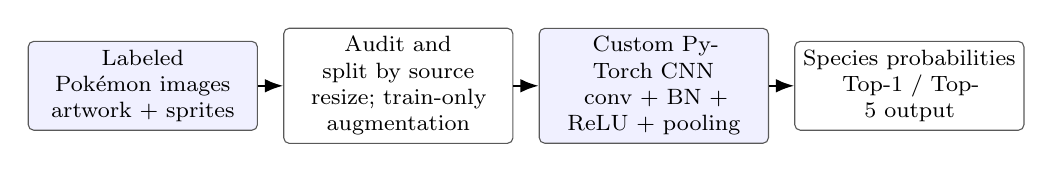
\begin{tikzpicture}[>=Latex, node distance=3.2mm, every node/.style={font=\footnotesize}, box/.style={draw=black!65,rounded corners=2pt,align=center,minimum height=0.65cm,text width=2.7cm,inner sep=3pt}]
\node[box,fill=blue!6] (a) {Labeled Pok\'emon images\\artwork + sprites};
\node[box,right=of a] (b) {Audit and split by source\\resize; train-only augmentation};
\node[box,right=of b,fill=blue!6] (c) {Custom PyTorch CNN\\conv + BN + ReLU + pooling};
\node[box,right=of c] (d) {Species probabilities\\Top-1 / Top-5 output};
\draw[->,thick] (a)--(b); \draw[->,thick] (b)--(c); \draw[->,thick] (c)--(d);
\end{tikzpicture}
\vspace{-2mm}
\caption{Proposed pipeline for single-Pok\'emon species classification. A HOG + linear SVM baseline uses the same held-out test images.}
\label{fig:pipeline}
\vspace{-3mm}
\end{figure}
\section*{Background \& Related Work}
AlexNet established the effectiveness of deep CNNs for large-scale visual recognition \citep{krizhevsky2012}; VGG showed the value of stacking small convolution filters \citep{simonyan2015}. ResNet introduced residual connections that help train deeper networks \citep{he2016}, while MobileNet explored lighter models with lower computation requirements \citep{howard2017}. These architectures motivate both our custom CNN blocks and an optional pretrained comparison, rather than treating an off-the-shelf model as the main contribution. Shorten and Khoshgoftaar survey image augmentation methods and their effect on generalization \citep{shorten2019}. We will test that idea specifically for variation between Pok\'emon artwork, sprites, and backgrounds, rather than assuming ordinary classification accuracy captures robustness.
\section*{Data Processing}
We plan to assemble a labeled image collection from the PokeAPI sprites repository (official-style artwork, HOME renders, and game sprites) \citep{pokeapiSprites} and The Complete Pok\'edex Dataset \citep{mitchellPokedex}. Pok\'edex numbers will provide consistent species IDs. First we will audit which species have multiple usable \emph{independent} images, remove broken files and duplicates (including perceptual near-duplicates), inspect ambiguous forms and incorrect labels, and document class counts and provenance. We will initially train on approximately 100--150 sufficiently represented species, increasing the count toward the full Pok\'edex only if coverage supports valid held-out evaluation. Images will be converted to RGB, padded/resized to $128\times128$, and normalized. We will split original image groups into 70\% train, 15\% validation, and 15\% test, grouping repeated or derived artwork together to prevent leakage. Only training images will receive rotations, colour jitter, blur, scaling, and background compositing. A separate test breakdown will report performance by source style. If a species lacks distinct source images for testing, we will flag it rather than claim reliable generalization.
\section*{Architecture}
Our main model will be a CNN coded in PyTorch, with three or four convolutional blocks (3$\times$3 convolutions, batch normalization, ReLU, and max pooling), global average pooling, dropout, and a final linear layer with one output per species. We will train using cross-entropy loss and Adam, select the learning rate and training duration using validation performance, and use early stopping to limit overfitting. We will compare training with and without augmentation while holding the architecture and test set fixed. Reported results will include Top-1 and Top-5 accuracy, macro-F1, confusion matrices, and per-style performance; we will also examine errors between visually similar species.
\section*{Baseline Model}
The primary baseline will extract histogram-of-oriented-gradients (HOG) features from the same resized images and train a linear support vector machine to predict species. We will select its regularization parameter on the validation set, then evaluate it on the identical untouched test set. This tests whether learned CNN features improve over a reproducible hand-crafted visual representation. If time permits, we will also report a fine-tuned ResNet-18 as an additional reference, not as a substitute for our own network.
\section*{Ethical Considerations}
Pok\'emon character images are copyrighted, so we will record sources, review permitted uses, and avoid redistributing image files without permission; any repository will prioritize code, labels/metadata where allowed, and download instructions. Uneven image availability across species and visual styles may favour popular Pok\'emon or clean artwork, so per-class and per-style results will accompany aggregate accuracy. Predictions may also be unreliable for fan art, alternate forms, or crowded scenes; this is a single-character classifier and should not be presented as a multi-object detector.
\newpage
\section*{References}
\begin{thebibliography}{99}
\bibitem[He et~al.(2016)]{he2016} K. He, X. Zhang, S. Ren, and J. Sun. Deep Residual Learning for Image Recognition. \emph{CVPR}, 2016.
\bibitem[Howard et~al.(2017)]{howard2017} A. G. Howard et al. MobileNets: Efficient Convolutional Neural Networks for Mobile Vision Applications. \emph{arXiv:1704.04861}, 2017.
\bibitem[Krizhevsky et~al.(2012)]{krizhevsky2012} A. Krizhevsky, I. Sutskever, and G. E. Hinton. ImageNet Classification with Deep Convolutional Neural Networks. \emph{NeurIPS}, 2012.
\bibitem[Mitchell(2026)]{mitchellPokedex} C. Mitchell. The Complete Pok\'edex Dataset. \url{https://github.com/cristobalmitchell/pokedex}, accessed October 2026.
\bibitem[PokeAPI Contributors(2026)]{pokeapiSprites} PokeAPI Contributors. Pok\'eAPI Sprites Repository. \url{https://github.com/PokeAPI/sprites}, accessed October 2026.
\bibitem[Shorten and Khoshgoftaar(2019)]{shorten2019} C. Shorten and T. M. Khoshgoftaar. A Survey on Image Data Augmentation for Deep Learning. \emph{Journal of Big Data}, 6(60), 2019.
\bibitem[Simonyan and Zisserman(2015)]{simonyan2015} K. Simonyan and A. Zisserman. Very Deep Convolutional Networks for Large-Scale Image Recognition. \emph{ICLR}, 2015.
\end{thebibliography}
\end{document}
